\hspace{0.5cm}


\section{Method to Extract \gones and \afone}  % The method to extract A1F1 is identical
 %\gones \g1wq}
\label{extraction}
%
\subsection{`Variation'' of the standard simulation}
\label{vari}


The whole chain of steps outlined in the previous sections for the standard simulation is repeated with just one major difference: the model input for the asymmetries $A_1$ for both the proton and the neutron are increased by a constant value\footnote{We arbitrarily chose 0.1 in the inelastic region, but could also have used any other value (not too big, however).} of 0.1. With all other model ingredients being kept constant, this change leads to a change of the spin structure function $g_1$ that can be straightforwardly calculated for each kinematic bin within the model:
\begin{equation}
\delta g_1(W,Q^2) = \delta A_1 \times F_1 \frac{\nu^2}{\nu^2 + Q^2}
\end{equation}

%===========  Count differences ======= 0
\begin{figure}[h] 
\centering
  %\leavevmode 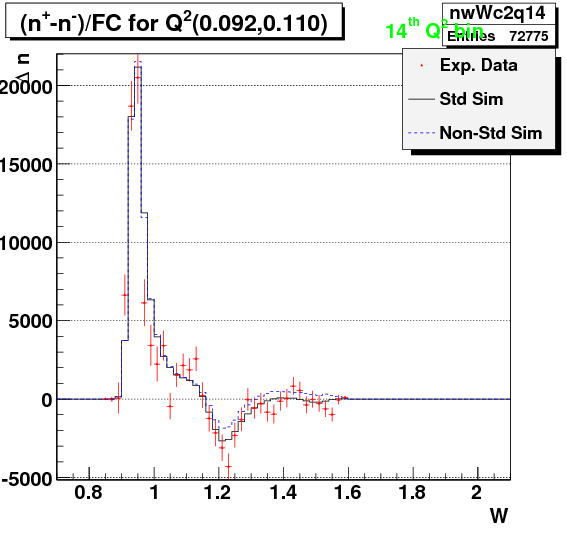
\includegraphics[width=0.9\textwidth]{figuresEG4/FigAnal/xsDiff_StdD57_nStdD68C194S139Eb7FewBins70Wbins.png} 
  \leavevmode 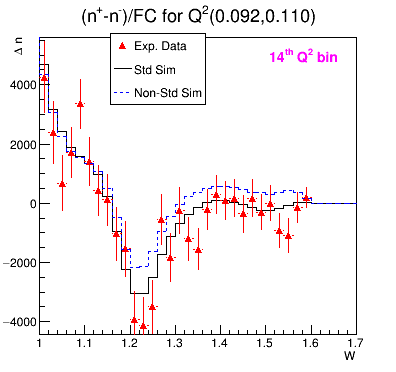
\includegraphics[width=0.9\textwidth]{figuresEG4/FigAnal/xsDiff_StdD79_nStdD80C71S181Eb7FewBins70WbinsZmd.png} 
  \caption[$\Delta n$ in one \qsqs bin (1.3 GeV)]{$\Delta n$ of experimental data and two versions of simulations in one particular \qsqs bin for 1.3 GeV case (for data on more \qsqs bins, see Fig. \ref{xsComp7}).}
  \label{xs1q7}  
\end{figure}




\begin{comment}  %Commented out on 12/4/13 (captions and references around this place was also modified somewhat.)
\begin{figure}[h] %ht, htpb (p - float, b = bottom, h=? t = top)
\centering
  \leavevmode 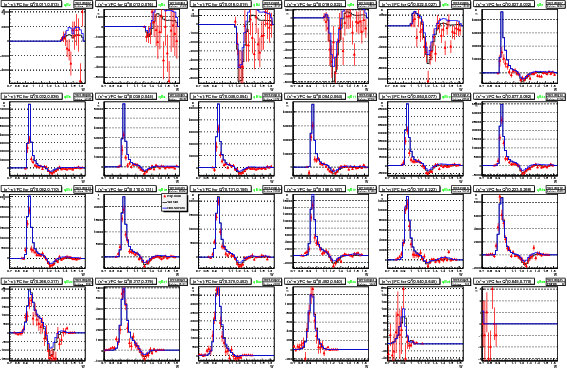
\includegraphics[width=1.0\textwidth]{figuresEG4/FigAnal/xsDiff_StdD57_nStdD68C194S139Eb7.png} 
  \caption[$\Delta n$ in all \qsqs bins (1.3 GeV)]{$\Delta n$ of experimental data and two versions of simulations in different \qsqs bins for 1.3 data.}
  \label{xs2sim7}  %http://wwwold.jlab.org/Hall-B//secure/eg4/adhikari/Analysis/SimStuffs/Extracted_g1/
\end{figure}


\begin{figure}[h] %ht, htpb (p - float, b = bottom, h=? t = top)
\centering
  \leavevmode 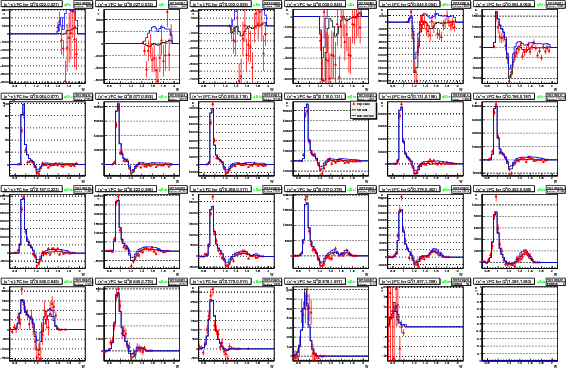
\includegraphics[width=1.0\textwidth]{figuresEG4/FigAnal/xsDiff_StdD57_nStdD62C194S139Eb8.png} 
  \caption[$\Delta n$ in all \qsqs bins (2.0 GeV)]{Same as Fig. \ref{xs2sim7} for the 2.0 data.} %{$\Delta n$ of experimental data and two versions of simulations in different \qsqs bins for 2.0 data.}
  \label{xs2sim8}  %http://wwwold.jlab.org/Hall-B//secure/eg4/adhikari/Analysis/SimStuffs/Extracted_g1/
\end{figure}
\end{comment}




Correspondingly, the simulated count difference $\Delta n (W,Q^2)$ will change to a new value $\Delta n'$. This ``non-standard'' simulation with $A_1 = A_1(standard) + 0.1$ is performed generating an about equal number of Monte-Carlo events. The final reconstructed data is then multiplied with the same overall scaling factor SF as for the standard simulation and then further (cross-)normalized by one additional factor $SF_{ext}=(\sigma^p_1/\sigma^p_2)/(N_1/N_2)$ to account for the change in cross section map and the (slight) difference in the number of the generated events between the standard and non-standard simulations. Here, $\sigma^p_1$ and $\sigma^p_2$ are the total cross sections for the positive $\Delta \sigma$ maps used for the standard and non-standard simulations and, $N_1$ and $N_2$ are the corresponding numbers of generated events. %In effect, the overall scale factor for the non-standard simulation is $SF_{ext}$ times what is used for the standard simulation. 
See Fig. (\ref{xs1q7}) to see how the polarized count differences look (in one particular \qsqs bin) in experimental and simulated data after such normalizations (for all other \qsqs bins, see Figs. \ref{xsComp7} and \ref{xsComp8}). %\ref{xs2sim7} and \ref{xs2sim8}).

% idea source: http://texblog.wordpress.com/2007/08/28/placing-figurestables-side-by-side-subfigure/ :Placing figures/tables side-by-side (\subfigure) Can include any number of figures/tables, not just two.
%http://wwwold.jlab.org/Hall-B//secure/eg4/adhikari/Analysis/SimStuffs/Extracted_g1/ResIfarm0901/EPSnw/
\begin{figure}[h]
\centering
\subfigure[\gones for standard and non-standard simulation]{
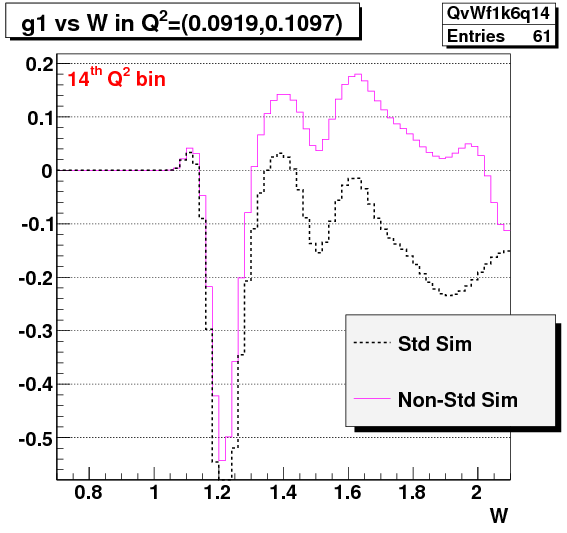
\includegraphics[scale=0.32]{figuresEG4/FigAnal/g1_stdNstd_Eb7FewBins.png}
\label{fig:twoG1}
}
\subfigure[Difference of the two \gone]{
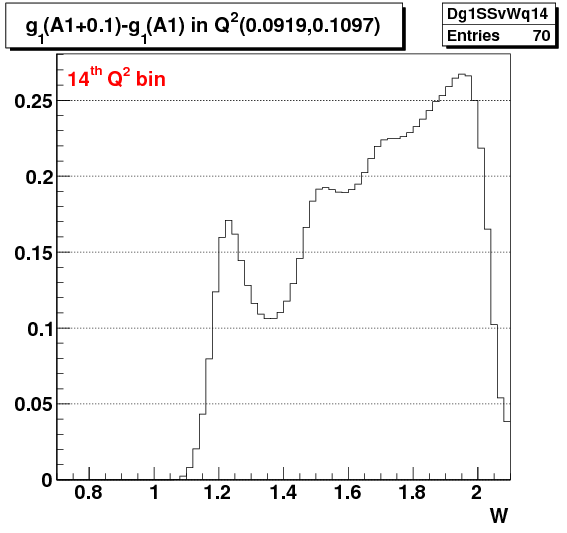
\includegraphics[scale=0.32]{figuresEG4/FigAnal/dg1_nStdNstd_Eb7FewBins.png}
\label{fig:DelG1}
}
\label{fig:g1Ch} %Effect of Dc-smear
\caption[Optional caption for list of figures]{Plots showing the change in model \gones due to the change of \aones to \aone + 0.1.}
\end{figure}


This change of the simulated $\Delta n (W,Q^2)$ to a new value $\Delta n'$ can be correlated to the increase in $g_1$ by solving for the two parameters $A$ and $B$ of the linear equation,
\begin{equation}
\Delta n(simul) = A + B\cdot \delta g_1,
\end{equation} %If an empty line is left below before 'where', the next line will be indented, because latex assumes that there is a new paragraph
where $A(W,Q^2) $ is the result for the simulated $\Delta n$ for the standard set of model inputs i.e., $A(W,Q^2)= \Delta n^{standard}(W,Q^2)$, and $B(W,Q^2) $ is the proportionality factor representing the change in $\Delta n(sim)$ per unit change in \gone, as given by:
\begin{equation}
\label{propFac}
B(W,Q^2)  = \frac{\Delta n' - \Delta n}{\delta g_1}.
\end{equation}

Similarly, in case of $A_1F_1$ evaluation, the factor is given by:
\begin{equation}
\label{propFacA1F1}
B(W,Q^2)  = \frac{\Delta n' - \Delta n}{\delta A_1F_1}.
\end{equation}


The proportionality factor  $B(W,Q^2)$ is then determined for each of the kinematic bins (in \wq) in which the experimental data has been histogrammed. For this purpose, using the RCSLACPOL program, we produce two values of structure function \gones in each kinematic bin - one is $g_1^{Standard}$ corresponding to the standard simulation and the other is $g_1^{non-standard}$ corresponding to the non-standard simulation. By dividing the above change in the count difference with the difference $\Delta g_1$ of these two structure functions, we get the factor $B(W,Q^2)$ for the bin. The similar procedure is followed to get the corresponding values of $B(W,Q^2)$ in the case of $A_1F_1$ evaluation.



\begin{figure}[h]
\centering
%===========  Delta n(non-std) - Delta n (std) =======3
\subfigure[Change in $\Delta n(sim)$ simulated count difference i.e. $\Delta N = \Delta n'(A_1+0.1) - \Delta n(A_1)$ due to the change of \aones to $A_1+0.1$ (for 1.3 GeV case).]{
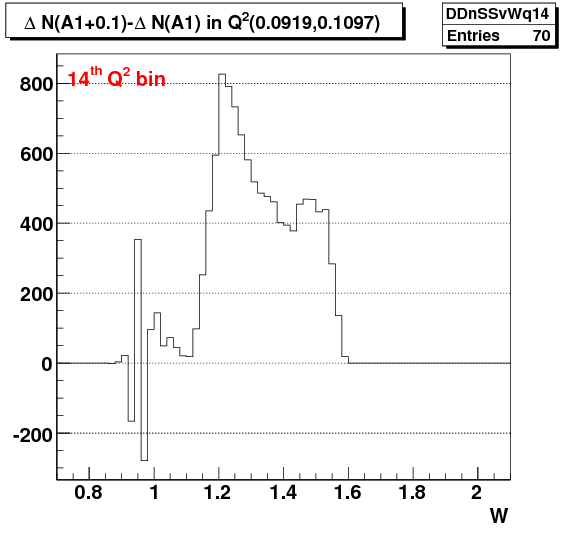
\includegraphics[scale=0.32]{figuresEG4/FigAnal/dDn_nStdNstd_Eb7FewBins.png}
\label{dDnSS7}
}
%===========  prop Fator =======5
\subfigure[Proportionality factor ($1/B(W,Q^2)$) for 1.3 GeV case. Black is the originial values. Red is the ones kept after discarding the first or last few (low statistics bins) that had unreasonably high (suddenly changing) ratios. This ensures we only show final data with ``good'' proportionality factor.]{
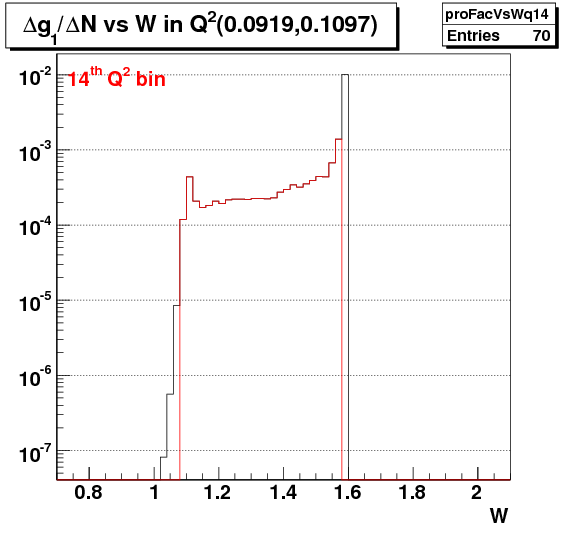
\includegraphics[scale=0.32]{figuresEG4/FigAnal/proportionalityFactorsEb7FewBins70Wbins.png}
\label{pFc1q7}
}
\label{dDnSnpFac} %Effect of Dc-smear
\caption[Optional caption for list of figures]{Plots for $\Delta n(sim)$ and the corresponding proportionality factors.}
\end{figure}




In principle (and ignoring the other enumerated possible sources of disagreement between data and simulation), we can then easily find the ``amount of change'' $\delta g_1$ to be added to the standard model $g_1$ to get perfect agreement:
\begin{equation}
\label{g1Ext}
% g_1^{extr}(W,Q^2) = g_1^{Standard} + \frac{\Delta n^{data}(W,Q^2) - \Delta n^{standard}(W,Q^2)}{B(W,Q^2) }
\delta g_1 = g_1^{extr}(W,Q^2) - g_1^{Standard} = \frac{\Delta n^{data}(W,Q^2) - \Delta n^{standard}(W,Q^2)}{B(W,Q^2) }
\end{equation}
where the values of $\Delta n^{data}$ and $\Delta n^{standard}$ come from the polarized count differences $\Delta n$ in the experimental data and the standard simulation respectively (as shown, for example, by the red points and black histograms in Fig. \ref{xs1q7} for one particular \qsqs bin). %figures \ref{xs2sim7} and \ref{xs2sim8}). %\textbf{\textcolor{red}{(I will update this work with results obtained with new tables for T1 and T2 which will be generated by turning off elastic/quasi-elastic part.)}} 

It is also straightforward to propagate the statistical uncertainty %error
to the extracted $g_1$. 
The statistical uncertainty in this extracted quantity totally comes from the uncertainty in the experimental counts $\Delta n^{data}$ (assuming there is no uncertainty in the model quantities involved and also in the simulation counts because we did our simulation with large enough statistics to warrant ignoring the uncertainties) as follows:
\begin{equation}
\label{g1ExtEr}
\sigma (g_1^{extr}(W,Q^2)) = \frac{\sigma(\Delta n^{data}(W,Q^2))}{B(W,Q^2) } .
\end{equation}
%The only thing remaining is the evaluation of systematic uncertainties due to the other possible sources of disagreement between data and simulation.

The values of \gones and its uncertainties thus extracted from 1.3 GeV data for one \qsqs bin is shown in Fig. (\ref{g1q7}). Similar results for all the bins from two beam energy data sets in different kinematic bins can be seen in Fig. \ref{extG1}.% (next chapter). 
%\textbf{\textcolor{red}{(Eventually, I will have one more plot that will have new data points that are calculated from the ones that were extracted separately from the two beam energy data sets.)}}




\begin{figure}[h]
\centering
%===========  Delta n(data) - Delta n (std) =======4
\subfigure[$\Delta n(data) - \Delta n(sim)$ (for 1.3 GeV case).]{
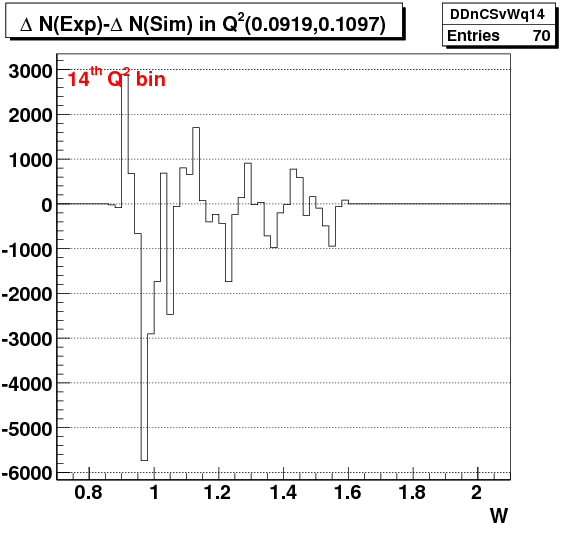
\includegraphics[scale=0.32]{figuresEG4/FigAnal/dDn_ExpNstd_Eb7FewBins.png}
\label{dDnCS7}
}
%===========  prop Fator =======5
\subfigure[Caculated \gones from 1.3 GeV data.]{
%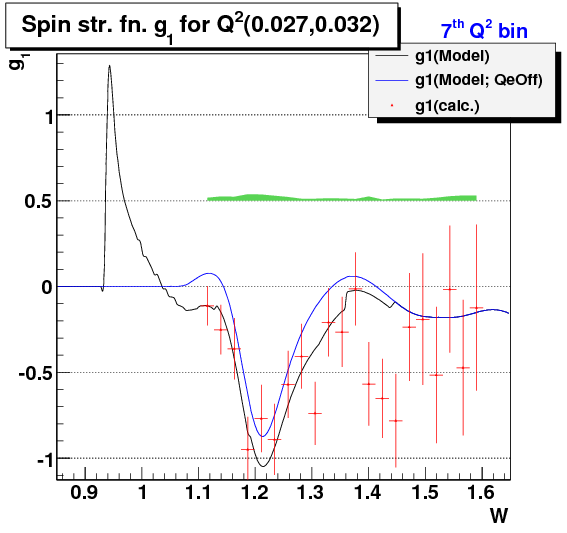
\includegraphics[scale=0.32]{figuresEG4/FigAnal/g1_stdAndExtracted_StdD57_nStdD68C194S139Eb7NoQeFewBins.png}
\includegraphics[scale=0.46]{figuresEG4/FigAnal/g1_stdAndExtracted_StdD79_nStdD80C71S181Eb7NoQeFewBins70Wbins.png}
\label{g1q7}
}
\label{dDnCSng1q7} %Effect of Dc-smear
\caption[Optional caption for list of figures]{Plots for $\Delta (\Delta n)$ and the corresponding extracted \gone. On the left, $\Delta (\Delta n)$ are the difference of the nomalized count differences  from the experimental and simulated (using 'standard' model) data. In other words, this gives the common numerator for Eqs. \ref{propFac} , \ref{propFacA1F1}. On the right, the blue line is that of the model $g_1$ that was used in the simulation when the quasi-elastic part was turned off. We used $g_1^{extracted} = g_1^{q.e. Off} + \delta g_1$ to get the measured $g_1$, where $\delta g_1$ is the calculated deviation (using Eq. \ref{g1Ext}) of the experimental $g_1$ from the model value which is derived from the deviation of the experimental polarized counts from the corresponding simulated counts.}
\end{figure}





%\subsection{Extraction of \afone} \label{exA1F1}
Because we are also interested in measuring the forward spin polarizability and the extended GDH integral, we also extract the product \afones which enters these integrals. We followed the exact same procedure for \gones as outlined above. %In this case, 
We determined new proportionality factors in each kinematic bin, again using Eq. \ref{propFac} as before but with the denominator replaced, this time, with the corresponding change in \afones (instead of the change in \gone). Then we can use the following expression (similar to equation \ref{g1Ext}) to extract \afonewq:

\begin{equation}
\label{a1f1Ext}
%A_{1}F_{1}^{extr}(W,Q^2) = A_{1}F_{1}^{Standard} + \frac{\Delta n^{data}(W,Q^2) - \Delta n^{standard}(W,Q^2)}{B_{A_1F_1}(W,Q^2) }
\delta A_{1}F_{1} = A_{1}F_{1}^{extr}(W,Q^2) - A_{1}F_{1}^{Standard} = \frac{\Delta n^{data}(W,Q^2) - \Delta n^{standard}(W,Q^2)}{B_{A_1F_1}(W,Q^2) }
\end{equation}

where
\begin{equation}
\label{propFac}
B_{A_1F_1}(W,Q^2)  = \frac{\Delta n' - \Delta n}{\delta A_1F_1}.
\end{equation}

And, the uncertainties on $A_1F_1$ can also be dealt in the same way as on \gone.

%Here, it is worth mentioning, once again, that the value of the proportionality factor $B(W,Q^2)$ involved in this case is different from what was used in extracting \gone.





%\subsection{Extraction of \gowq}
%\label{exG1}

%In this section, the methods to extract \gone and evaluate its uncertainties are described.  %$g_{1}$

%The ``non-standard'' simulation with $A_1 = A_1(standard) + 0.1$ (as mentioned above in section \ref{vari}) is performed with an about equal number of Monte-Carlo events generated at the start of the simulation chain. The final reconstructed data is then multiplied with the same overall scaling factor SF and further cross-normalized with the standard simulation by one extra factor $SF_{ext}=(\sigma^p_2/\sigma^p_2)/(N_1/N_2)$ to account for their different cross sections and the different number of events initially generated for each case, where $\sigma^p_1$ and $\sigma^p_2$ are the total cross sections for the positive polarization maps used for the standard and non-standard simulations and, likewise, $N_1$ and $N_2$ are the corresponding numbers of events initially generated for the two simulations. In effect, the overall scale factor for the non-standard simulation is $SF_{ext}$ times what is used for the standard simulation. See Fig. (\ref{xs1q7}) to see how the polarized count differences look (in one particular \qsqs bin) in experimental and simulated data after such normalizations (for all other \qsqs bins, see figures \ref{xs2sim7} and \ref{xs2sim8}). %SF=(xsMapTotPosPol2/xsMapTotPosPol)*(pFlNum*1.0/pFlNum2);   (In a previous section on data-sim comparison, I think, I should give a little detail/equation/expression on somewhat similar normalization of -ve polarization simulation with respect to the +ve polarization simulation to get the final overall polarized simulated data.)




%\input{chap4simul/g1EtcExtractionAuxi1.tex} %Many plots in Single Q2 bins (moved used content of this file here on 12/4/13)

%===========  g1(non-std), g1(std) and the difference ======= 1




%\textbf{\textcolor{red}{I think, above two plots shouldn't depend on beam energy, but due to acceptance constraints, only the shown bins receive the corresponding EG4 data. That's should explain the distinction, because we produced model values only in the region covered by EG4.}}

%===========  Delta n(non-std) - Delta n (std) =======3









